% Options for packages loaded elsewhere
\PassOptionsToPackage{unicode}{hyperref}
\PassOptionsToPackage{hyphens}{url}
\documentclass[
  ignorenonframetext,
]{beamer}
\newif\ifbibliography
\usepackage{pgfpages}
\setbeamertemplate{caption}[numbered]
\setbeamertemplate{caption label separator}{: }
\setbeamercolor{caption name}{fg=normal text.fg}
\beamertemplatenavigationsymbolsempty
% remove section numbering
\setbeamertemplate{part page}{
  \centering
  \begin{beamercolorbox}[sep=16pt,center]{part title}
    \usebeamerfont{part title}\insertpart\par
  \end{beamercolorbox}
}
\setbeamertemplate{section page}{
  \centering
  \begin{beamercolorbox}[sep=12pt,center]{section title}
    \usebeamerfont{section title}\insertsection\par
  \end{beamercolorbox}
}
\setbeamertemplate{subsection page}{
  \centering
  \begin{beamercolorbox}[sep=8pt,center]{subsection title}
    \usebeamerfont{subsection title}\insertsubsection\par
  \end{beamercolorbox}
}
% Prevent slide breaks in the middle of a paragraph
\widowpenalties 1 10000
\raggedbottom
\AtBeginPart{
  \frame{\partpage}
}
\AtBeginSection{
  \ifbibliography
  \else
    \frame{\sectionpage}
  \fi
}
\AtBeginSubsection{
  \frame{\subsectionpage}
}
\usepackage{iftex}
\ifPDFTeX
  \usepackage[T1]{fontenc}
  \usepackage[utf8]{inputenc}
  \usepackage{textcomp} % provide euro and other symbols
\else % if luatex or xetex
  \usepackage{unicode-math} % this also loads fontspec
  \defaultfontfeatures{Scale=MatchLowercase}
  \defaultfontfeatures[\rmfamily]{Ligatures=TeX,Scale=1}
\fi
\usepackage{lmodern}
\ifPDFTeX\else
  % xetex/luatex font selection
\fi
% Use upquote if available, for straight quotes in verbatim environments
\IfFileExists{upquote.sty}{\usepackage{upquote}}{}
\IfFileExists{microtype.sty}{% use microtype if available
  \usepackage[]{microtype}
  \UseMicrotypeSet[protrusion]{basicmath} % disable protrusion for tt fonts
}{}
\makeatletter
\@ifundefined{KOMAClassName}{% if non-KOMA class
  \IfFileExists{parskip.sty}{%
    \usepackage{parskip}
  }{% else
    \setlength{\parindent}{0pt}
    \setlength{\parskip}{6pt plus 2pt minus 1pt}}
}{% if KOMA class
  \KOMAoptions{parskip=half}}
\makeatother
\usepackage{longtable,booktabs,array}
\newcounter{none} % for unnumbered tables
\usepackage{calc} % for calculating minipage widths
\usepackage{caption}
% Make caption package work with longtable
\makeatletter
\def\fnum@table{\tablename~\thetable}
\makeatother
\usepackage{graphicx}
\makeatletter
\newsavebox\pandoc@box
\newcommand*\pandocbounded[1]{% scales image to fit in text height/width
  \sbox\pandoc@box{#1}%
  \Gscale@div\@tempa{\textheight}{\dimexpr\ht\pandoc@box+\dp\pandoc@box\relax}%
  \Gscale@div\@tempb{\linewidth}{\wd\pandoc@box}%
  \ifdim\@tempb\p@<\@tempa\p@\let\@tempa\@tempb\fi% select the smaller of both
  \ifdim\@tempa\p@<\p@\scalebox{\@tempa}{\usebox\pandoc@box}%
  \else\usebox{\pandoc@box}%
  \fi%
}
% Set default figure placement to htbp
\def\fps@figure{htbp}
\makeatother
\setlength{\emergencystretch}{3em} % prevent overfull lines
\providecommand{\tightlist}{%
  \setlength{\itemsep}{0pt}\setlength{\parskip}{0pt}}
% Slide layout defaults for warning-clean scientific decks.
\usepackage{etoolbox}
\IfFileExists{xurl.sty}{\usepackage{xurl}}{}
\IfFileExists{seqsplit.sty}{\usepackage{seqsplit}}{\newcommand{\seqsplit}[1]{#1}}
\protected\def\breakseq#1{\seqsplit{#1}}
\protected\def\breaktt#1{\begingroup\ttfamily\seqsplit{#1}\endgroup}
\setlength{\emergencystretch}{6em}
\tolerance=5000
\hbadness=10000
\hfuzz=1pt
\setlength{\tabcolsep}{2pt}
\AtBeginEnvironment{longtable}{\tiny\renewcommand{\arraystretch}{0.86}\setlength{\tabcolsep}{1pt}}
\AtBeginEnvironment{tabular}{\tiny\renewcommand{\arraystretch}{0.86}\setlength{\tabcolsep}{1pt}}

% Natbib and cross-reference fallbacks — slides don't load natbib
% or cleveref, but combined-PDF manuscript prose may emit these
% commands. The fallback renders citations as a bracketed key list
% and cross-references as detokenized labels so slides don't fail on
% undefined control sequences or raw underscores. \providecommand is
% a no-op if packages load later.
\providecommand{\citep}[1]{[#1]}
\providecommand{\citet}[1]{#1}
\providecommand{\citealp}[1]{#1}
\providecommand{\citeauthor}[1]{#1}
\providecommand{\citeyear}[1]{#1}
\providecommand{\cref}[1]{\texttt{\detokenize{#1}}}
\providecommand{\Cref}[1]{\texttt{\detokenize{#1}}}
\usepackage{bookmark}
\IfFileExists{xurl.sty}{\usepackage{xurl}}{} % add URL line breaks if available
\urlstyle{same}
% fallback for those not using the hyperref driver hyperxmp:
\makeatletter
\@ifundefined{xmpquote}{\newcommand{\xmpquote}[1]{#1}}{}
\makeatother
\hypersetup{
  hidelinks,
  pdfcreator={LaTeX via pandoc}}

\author{\texorpdfstring{}{}}
\date{}

\begin{document}

\section{Results: Citation Network}\label{results-citation-network}

\begin{frame}[allowframebreaks]{RQ4: Citation Geometry}
\protect\phantomsection\label{rq4-citation-geometry}
Resolving each record's references against the corpus yields an
intra-corpus citation graph (built and analyzed with NetworkX
\breakseq{[@hagberg2008exploring]}) of 2204 nodes and 8,772 edges across 1371
connected components, with a graph density of 0.18\% and a mean
in-degree of 4.0. Of 38,802 total outgoing references, 22.6\% resolve to
another record inside the corpus --- a resolution rate that reflects how
self-contained the retrieved slice of the literature is rather than the
underlying citation density of any single work.

The citation network has 1377 communities (detected by modularity
optimization), a maximum in-degree of 165 (the most-cited paper within
the corpus), and a maximum out-degree of 145 (the paper that cites the
most other corpus members).
\end{frame}

\begin{frame}[allowframebreaks]{Centrality Analysis}
\protect\phantomsection\label{centrality-analysis}
Centrality scores (PageRank \breakseq{[@page1999pagerank]} and HITS) and
modularity-based community detection \breakseq{[@clauset2004finding]} are
rounded and ranked with a stable tiebreaker so the reported hub and
authority rankings are byte-reproducible across runs despite the
floating-point non-associativity of the underlying iterative solvers.

\textbf{Table 4. Top 5 papers by PageRank.}

{\def\LTcaptype{none} % do not increment counter
\begin{longtable}[]{@{}lll@{}}
\toprule\noalign{}
Rank & DOI & PageRank \\
\midrule\noalign{}
\endhead
1 & 10.1177/026988110001400107 & 0.036955 \\
2 & 10.1212/wnl.54.5.1166 & 0.027240 \\
3 & 10.1523/jneurosci.21-05-01787.2001 & 0.013811 \\
4 & 10.1523/jneurosci.20-22-08620.2000 & 0.011443 \\
5 & 10.4088/jcp.v61n0510 & 0.008104 \\
\bottomrule\noalign{}
\end{longtable}
}

\textbf{Table 5. Top 5 authority papers (HITS).}

{\def\LTcaptype{none} % do not increment counter
\begin{longtable}[]{@{}lll@{}}
\toprule\noalign{}
Rank & DOI & Authority \\
\midrule\noalign{}
\endhead
1 & 10.1038/sj.npp.1301534 & 0.017582 \\
2 & 10.1007/s00213-002-1250-8 & 0.015979 \\
3 & 10.1124/jpet.106.106583 & 0.015039 \\
4 & 10.1001/jama.2009.351 & 0.014535 \\
5 & 10.1523/jneurosci.21-05-01787.2001 & 0.014289 \\
\bottomrule\noalign{}
\end{longtable}
}

\textbf{Table 6. Top 5 hub papers (HITS).}

{\def\LTcaptype{none} % do not increment counter
\begin{longtable}[]{@{}lll@{}}
\toprule\noalign{}
Rank & DOI & Hub \\
\midrule\noalign{}
\endhead
1 & 10.3389/fnins.2021.656475 & 0.012064 \\
2 & 10.1016/bs.apha.2023.10.006 & 0.011690 \\
3 & 10.1038/sj.npp.1301534 & 0.010781 \\
4 & 10.1080/08897077.2019.1700584 & 0.010618 \\
5 & 10.1007/s00213-013-3232-4 & 0.009971 \\
\bottomrule\noalign{}
\end{longtable}
}

The most influential paper by PageRank (DOI 10.1177/026988110001400107)
is a foundational work that anchors the citation structure --- its high
authority score confirms it is frequently cited by other corpus members.
Hub papers, which cite many other corpus members, serve as integrative
reviews or meta-analyses that connect disparate threads of the
literature.

\pandocbounded{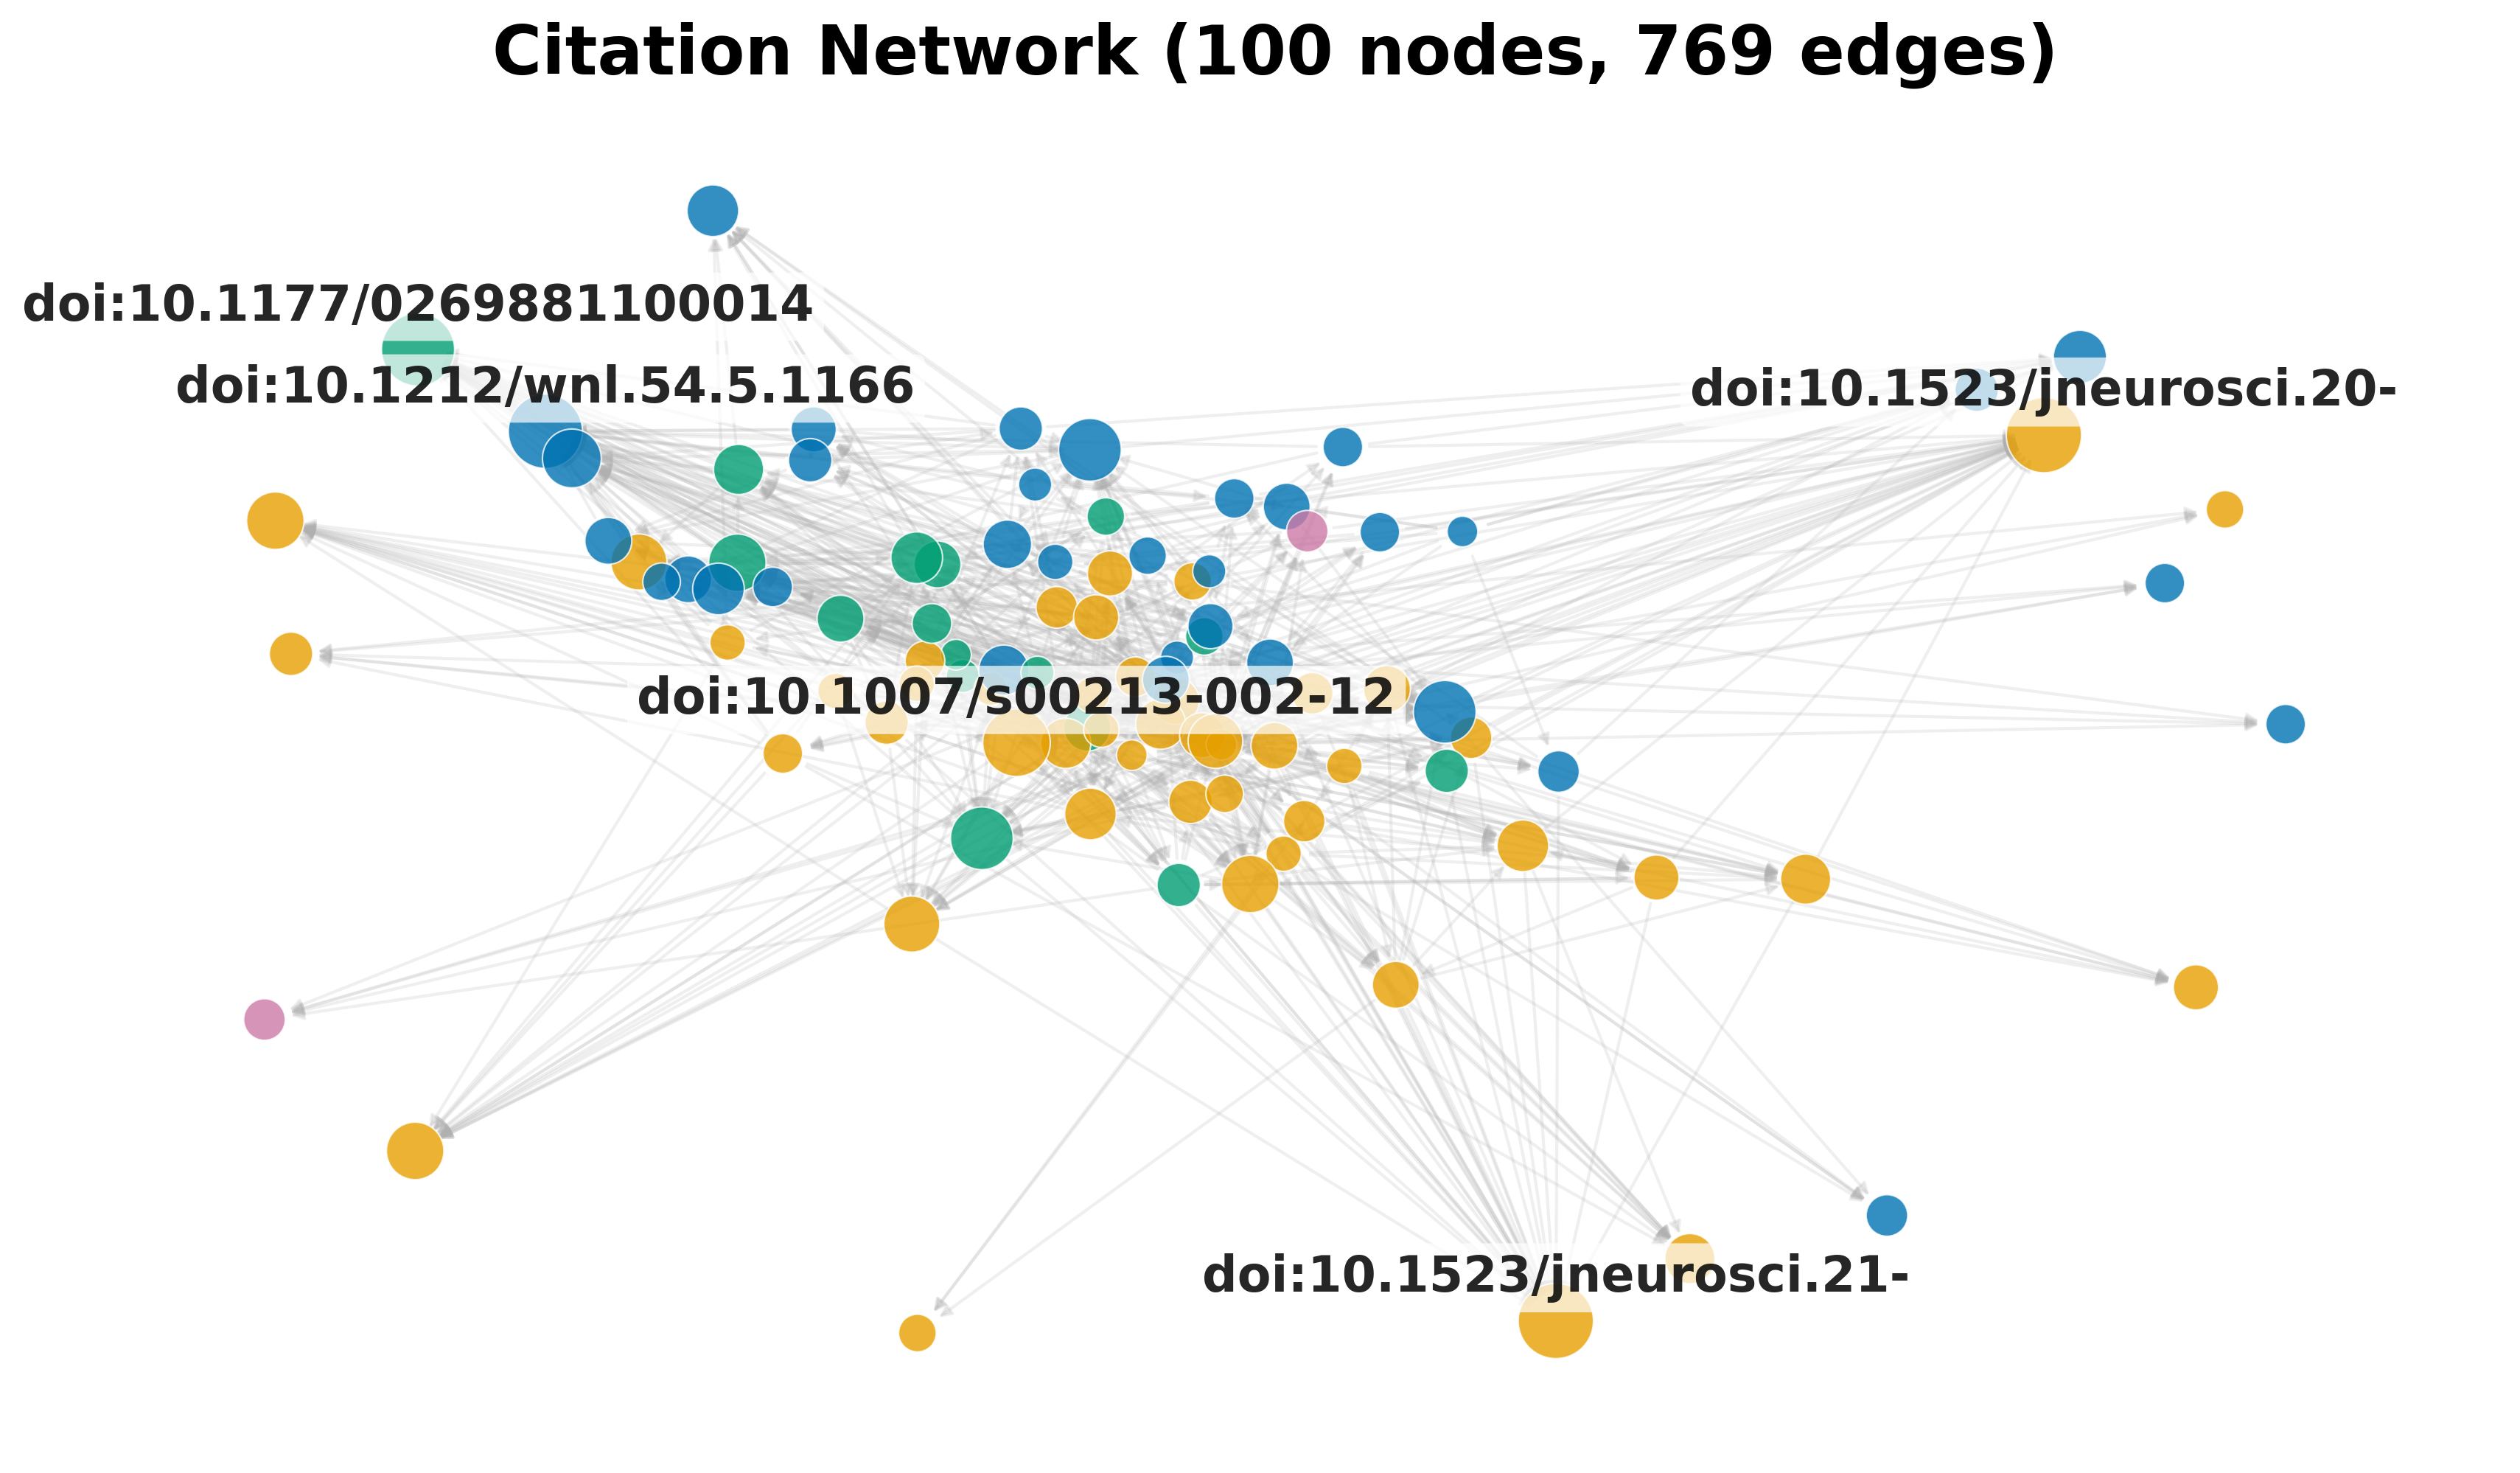
\includegraphics[keepaspectratio,alt={Citation network for Modafinil. Nodes represent papers; directed edges represent citation links. Node colours indicate community membership (1377 communities detected by modularity optimization). Layout uses a spring-based algorithm with a fixed seed for reproducibility.}]{../figures/citation_network.png}}\{\{\#fig:citation\_network\}\}

\pandocbounded{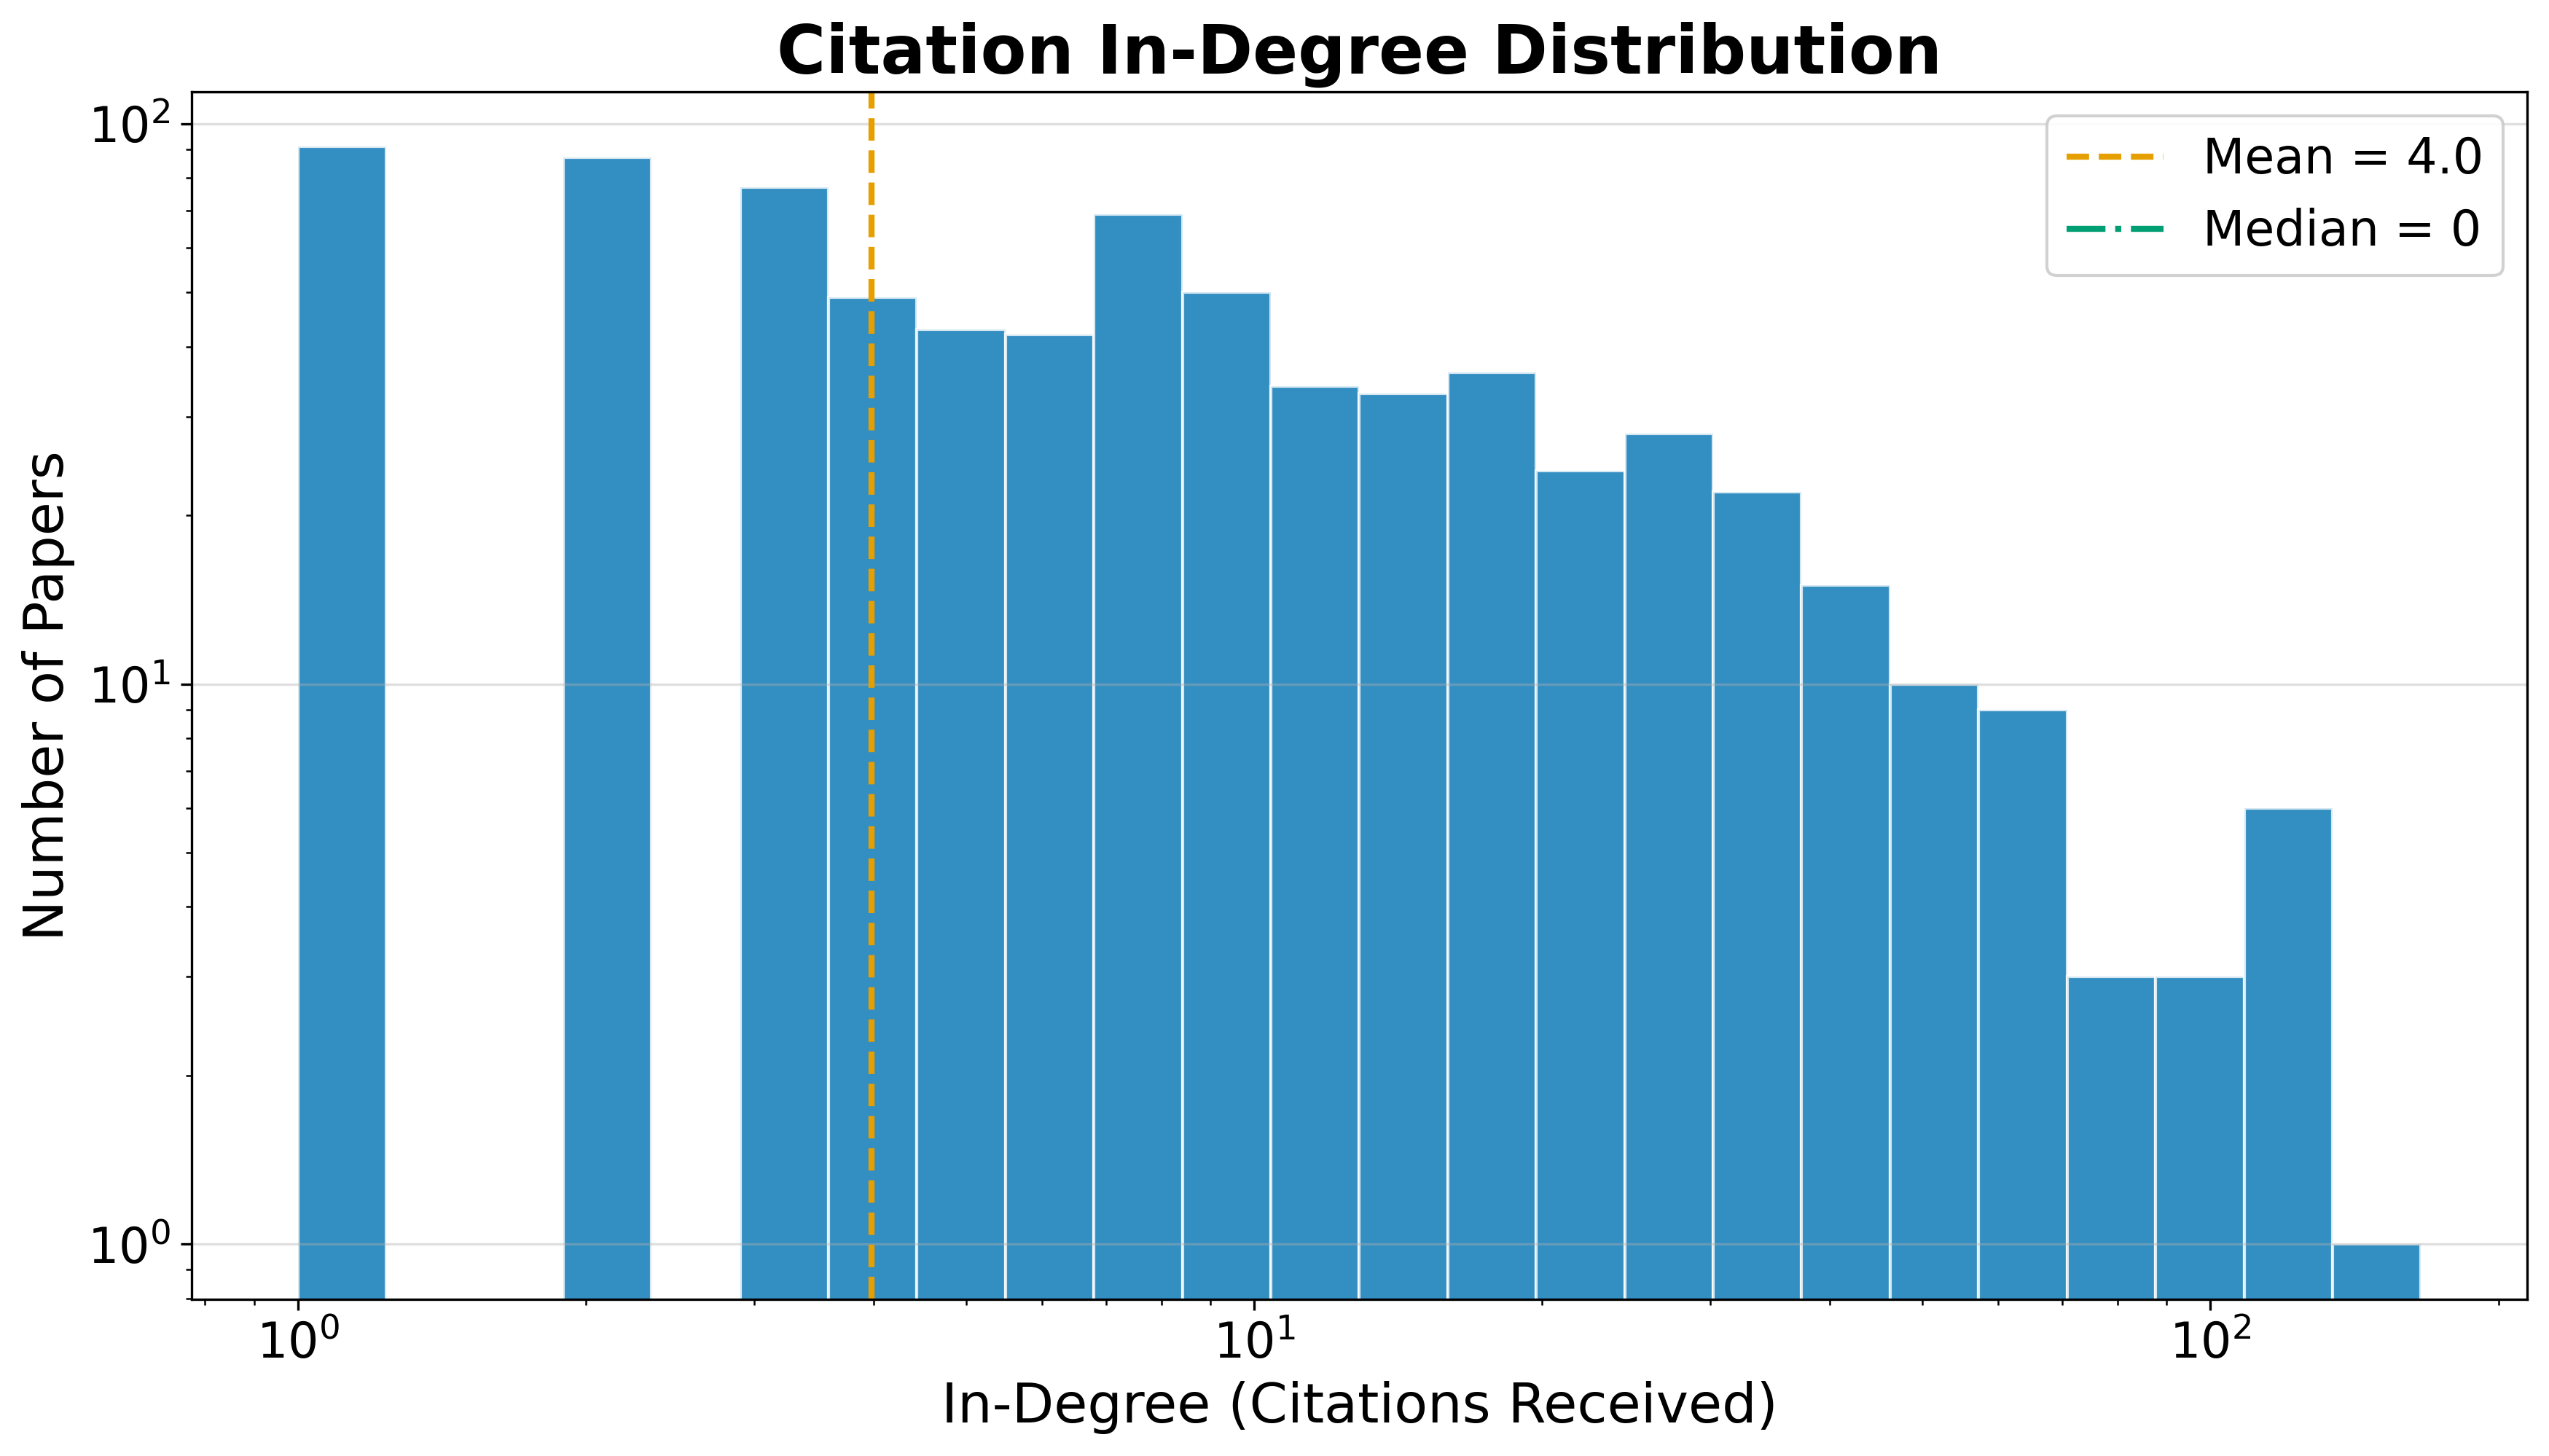
\includegraphics[keepaspectratio,alt={Degree distribution for the Modafinil citation network. The histogram shows the frequency of each in-degree value on a log-linear scale, revealing the heavy-tailed structure characteristic of citation networks.}]{../figures/degree_distribution.png}}\{\{\#fig:degree\_distribution\}\}

The heavy-tailed degree distribution is characteristic of citation
networks: a small number of highly-cited papers anchor the structure,
while the long tail of low-degree nodes represents newer or peripheral
works. The low graph density (0.18\%) reflects the sparsity of
intra-corpus citation links --- most papers cite works outside the
retrieved slice, which is expected for a max-results-capped retrieval.
\end{frame}

\begin{frame}[allowframebreaks]{Advanced Network Metrics}
\protect\phantomsection\label{advanced-network-metrics}
Beyond PageRank and HITS, the network analysis computes betweenness
centrality (which papers bridge different communities), closeness
centrality (which papers are near all others), degree assortativity (do
highly-cited papers cite other highly-cited papers?), and average
clustering coefficient (how tightly knit are local neighborhoods).

The degree assortativity coefficient is -0.0579, and the average
clustering coefficient is 0.1047. A negative assortativity indicates
that highly-cited papers tend to cite less-cited papers (dissortative
mixing), which is typical of citation networks where review papers (high
in-degree) cite many primary studies (low in-degree).

\textbf{Table 7. Top 5 papers by betweenness centrality.}

{\def\LTcaptype{none} % do not increment counter
\begin{longtable}[]{@{}lll@{}}
\toprule\noalign{}
Rank & DOI & Betweenness \\
\midrule\noalign{}
\endhead
1 & 10.1038/sj.npp.1301534 & 0.006017 \\
2 & 10.4088/jcp.v67n0406 & 0.003330 \\
3 & 10.2165/00003495-200868130-00003 & 0.002036 \\
4 & 10.1124/jpet.106.106583 & 0.001949 \\
5 & 10.1007/s00213-005-0044-1 & 0.001899 \\
\bottomrule\noalign{}
\end{longtable}
}

Papers with high betweenness centrality serve as bridges between
different topical communities in the citation network --- their removal
would fragment the graph into disconnected components. These bridging
papers are often review articles or methodological papers that connect
disparate research threads.
\end{frame}

\end{document}
